\documentclass{article}
\usepackage{graphicx}
\graphicspath{ {images/} }
\usepackage[utf8]{inputenc}
\usepackage{listings}

\title{Programa 1 - Universo}
\author{Leon Tejeda 2CM5}
\date{Octubre 2020}

\begin{document}
\maketitle
\begin{flushleft}
Se nos dejo la tarea de hacer un programa que imprima en manera de conjunto todo el universo de cadenas binarias de un largo dado

INTRODUCCION:

Primero empezaremos definiendo que es un numero binario: 	Un numero binario se representa por unicamente 0's y 1's, cualquier numero se puede representar mediante este sistema de numeros.

Universo de cadenas binarias:	Para entender el problema, es necesario entender que un universo de cadenas binarias, contiene a todas las cadenas binarias de todos los argos hasta el largo dado.

					Esto quiere decir que se tendran 2 \^{}  n + 2  \^{}  (n-1) + 2  \^{}  (n-2) + ... + 2 + 1 

PLANTEAMIENTO DEL PROBLEMA:

Programar el universo de las cadenas binarias (Sigma \^{} n). Dada una "n" que introduzca el usuario o que el programa lo determine automáticamente. El rango de "n" debe de estar en el intervalo de [0,1000].

1. El programa debe de preguntar si quiere calcular otra "n" o no.

2. La salida, expresada en notación de conjunto, debe ir a un archivo de texto.

3. Una segunda salida (archivo de texto) debe concatenar todas las cadenas calculadas en una sola cadena, quitar las llaves, comas y cualquier otro símbolo que no sean 0s y 1s.

4. Del primer archivo de salida, graficar el número de 1s de cada cadena. El eje de las x es la cadena y el eje de las y el número de 1s que tiene esa cadena. Específicamente, calcular y graficar cuando n=23. Al mismo tiempo, calcular la gráfica pero calculando su logaritmo en base 2 y 10 respectivamente.

5. Del segundo archivo de salida, particionar la cadena en subcadenas de longitud 32 y graficar la cantidad de unos de esas subcadenas. Al mismo tiempo, calcular la gráfica pero calculando su logaritmo en base 2 y 10 respectivamente.
IMPLEMENTACION:

Implementamos un algoritmo que convierta los numeros decimales a binarios

Despues rellenamos el numero con ceros dependiendo del largo necesario, para llegar al largo necesario

Se contabilizo el numero de 1's que tenia el numero y se checo el numero de la cadena, esto se guardo en un arcchivo como coordenadas y la cadena se guardo en un arcivo como conjunto

Al graficar se tomo en cuenta el numero de 1's como las y's y el numero de la cadena como 0's

Codigo:

\begin{lstlisting}

import random
import os
import math
import cmath
from matplotlib import pyplot

#Primera Grafica
def pasar_coordenadas1(x, y):
    archivo = open("Programa1_Coordenadas1.txt", "a")
    archivo.write(str(x))
    archivo.write(",")
    archivo.write(str(y))
    archivo.write("\n")
    archivo.close()
    

#Segunda Grafica (32 bits)
def pasar_coordenadas2(x,y):
    archivo = open("Programa1_Coordenadas2.txt", "a")
    archivo.write(str(x))
    archivo.write(",")
    archivo.write(str(y))
    archivo.write("\n")
    archivo.close()
    

def grafica1(k):
     
    archivo = open("Programa1_Coordenadas1.txt", "r")
    for coordenada in archivo:
        x = False
        y = False
        separacion = False
        
        for dato in coordenada:
            if dato != "," and dato !=" " and separacion == False:
                if x == False:
                    x = dato
                
                else:
                    x = x + dato
            
            elif dato != "," and dato !=" " and separacion == True:
                if y == False:
                    y = dato
                
                else:
                    y = y + dato
            else:
                separacion = True
                
        pyplot.plot(int(x), int(y), marker=".", color="blue")
        
        # Logaritmo base 2
        if int(y) != 0:
            y2 = math.log2(int(y))
        else:
            y2=0
            
        pyplot.plot(int(x), y2, marker=".", color="red")

        # Logaritmo base 10
        if int(y) != 0:
            y10 = math.log10(int(y))
        else:
            y10=0
            
        pyplot.plot(int(x), y10, marker=".", color="green")
                
                
    # Establecer el color de los ejes.
    pyplot.axhline(0, color="black")
    pyplot.axvline(0, color="black")
    
    # Limitar los valores de los ejes.
    pyplot.xlim(0, 2**k)
    pyplot.ylim(0, k)
    
    #Salva la Grafica
    pyplot.savefig("Programa1_Grafica1.png")
    
    # Mostrarlo.
    #pyplot.show()

            
    archivo.close()
    
    
    
def grafica2(k):
    #print("Aqui va la grafica2")
    archivo = open("Programa1_Coordenadas2.txt", "r")
    for coordenada in archivo:
        x = False
        y = False
        separacion = False
        
        for dato in coordenada:
            if dato != "," and dato !=" " and separacion == False:
                if x == False:
                    x = dato
                
                else:
                    x = x + dato
            
            elif dato != "," and dato !=" " and separacion == True:
                if y == False:
                    y = dato
                
                else:
                    y = y + dato
            else:
                separacion = True
                
        pyplot.plot(int(x), int(y), marker=".", color="blue")
        
        # Logaritmo base 2
        if int(y) != 0:
            y2 = math.log2(int(y))
        else:
            y2=0
            
        pyplot.plot(int(x), y2, marker=".", color="red")

        # Logaritmo base 10
        if int(y) != 0:
            y10 = math.log10(int(y))
        else:
            y10=0
            
        pyplot.plot(int(x), y10, marker=".", color="green")
                
    
    # Establecer el color de los ejes.
    pyplot.axhline(0, color="black")
    pyplot.axvline(0, color="black")
    
    # Limitar los valores de los ejes.
    pyplot.xlim(0, 2**k)
    pyplot.ylim(0, 32)
    
    #Salva la Grafica
    pyplot.savefig("Programa1_Grafica2.png")
    
    # Mostrarlo.
    #pyplot.show()
    archivo.close()
    

#cuenta cuantos 1s hay en el numero binario
def unos(numero):

    unos = 0
    if numero >= 1:
        while numero > 1:
                
            residuo = numero % 2
            numero = numero // 2
                
            if residuo == 1:
                unos = unos + 1
        
        unos = unos + 1
                            
    return unos

#Transformador (Binario-Decimal)
def trans_decimal(cadena):
    numero = 0
    posicion = len(cadena)-1

    while posicion > -1:
        aux = (len(cadena)-1) - posicion
        if cadena[posicion] == "1" and numero == 0:
            numero = 2 ** aux
        elif cadena[posicion] == "1":
            numero = numero + (2**aux)
            
        posicion = posicion - 1
    return numero


#Transformador (Deccimal-Binario)
def trans_binario(numero):
    binario = 0

    #print ("Transformando a binario....")

    if numero > 1:
        while numero > 1:
                
            residuo = numero % 2
            numero = numero // 2
                
            if binario == 0:
                binario = str(residuo)
                    
            else:
                binario = str(residuo) + binario
        
        binario = str(numero) + binario
                
    else:
        binario = str(numero)
        
    return binario

def relleno(cadena, largo):
    
    if(largo == len(cadena)):
        return cadena
    else:
        for x in range (0, largo - len(cadena)):
            cadena = "0" + cadena
            
    return cadena


#Archivo 1 (Forma de Conjunto)
def pasarlo_archivo1(binario, k):
    archivo = open("Programa1_Archivo1.txt", "a")
    
    if k == 0:
        archivo.write("{")
        archivo.write("e")
        
    else:
        archivo.write(" ,")
        archivo.write(binario)
        
    archivo.close()
        

#Archivo2 (Forma de cadena)
def pasarlo_archivo2(binario, k):
    archivo = open("Programa1_Archivo2.txt", "a")
    
    if k != 0:
        archivo.write(binario)    
    
    archivo.close()

#Archivo2 (Separacion de 32 bits)
def separador_de_32_bits_archivo2():
    contador = 0
    binario = 0
    archivo = open("Programa1_Archivo2.txt", "r")
    
    for linea in archivo:
        for caracter in linea:
            if contador < 31 and binario == 0:
                binario = caracter
                contador = contador + 1
                
            elif contador < 31:
                binario = binario + caracter
                contador = contador + 1
            
            else:
                contador = 0
                binario = binario + ","
                binario = binario + caracter
    archivo.close()
    binario = binario + ","
    return binario


def borrar_archivo_existente():
    archivo = open("Programa1_Archivo1.txt", "w")
    archivo.close()
    
    archivo = open("Programa1_Coordenadas1.txt", "w")
    archivo.close()
    
    archivo = open("Programa1_Archivo2.txt", "w")
    archivo.close()
    
    archivo = open("Programa1_Coordenadas2.txt", "w")
    archivo.close()
    

def universo(k):
    
    coordenada_x = 0
    coordenada_x1 = 1
    coordenada_y1 = 0
    
    for i in range (0, k+1):
        largo = 2 ** i
        
        for j in range(0, largo):
            #Trancformaiocn a binario y Relleno de 0
            binario = trans_binario(j)
            binario = relleno(binario, i)
            
            #Escritura Archivo1
            pasarlo_archivo1(binario, i)
            
            #Coordenadas de la Primera Grafica
            coordenada_y = unos(j)
            pasar_coordenadas1(coordenada_x, coordenada_y)
            coordenada_x = coordenada_x + 1
            
            #Escritura Archivo2
            pasarlo_archivo2(binario, i)
            
    archivo = open("Programa1_Archivo1.txt", "a")
    archivo.write("}")
    archivo.close()
    
    aux=separador_de_32_bits_archivo2()
    archivo = open("Programa1_Archivo2.txt", "w")
    archivo.write(aux)
    archivo.close()
    
    #Coordenadas de la Segunda Grafica
    archivo = open("Programa1_Coordenadas2.txt", "w")
    for caracter in aux:
        if caracter == ",":
            coordenada_y1 = trans_decimal(coordenada_y1)
            coordenada_y1 = unos(int(coordenada_y1))
            
            pasar_coordenadas2(coordenada_x1, coordenada_y1)
            coordenada_x1 = coordenada_x1 + 1
            coordenada_y1 = 0
        
        elif coordenada_y1 == 0:
            coordenada_y1 = caracter
            
        else:
            coordenada_y1 = coordenada_y1 + caracter
                
    archivo.close()
    
    grafica1(k)
    grafica2(k)


def menu():
    print("Seleccione una opcion")
    print("1. Ingresar un numero entre 0-1000")
    print("2. Generar un numero aleatorio entre 0-1000")

    op = int(input(""))

    if op == 1:
        print("Ingrese un numero entre 0-1000")
        k = int(input(""))
        universo(k)
        
    elif op == 2:
        k = random.randint(0, 1000)
        print("El numero aleatorio es igual a: " + str(k))
        universo(k)
        
    else:
        print("Ingrese un numero valido")


repetir = 1

while repetir == 1:
    borrar_archivo_existente()
    menu()
    print("Si desea ingresar otro numero presione (y)")
    respuesta = input("")
    os.system("cls")
    
    if respuesta != 'y' and respuesta != 'Y':
        repetir = 0 

\end{lstlisting}

FUNCIONAMIENTO:

Cuando n=23

Esta es la forma e la que imprime los datos en forma de conjuto
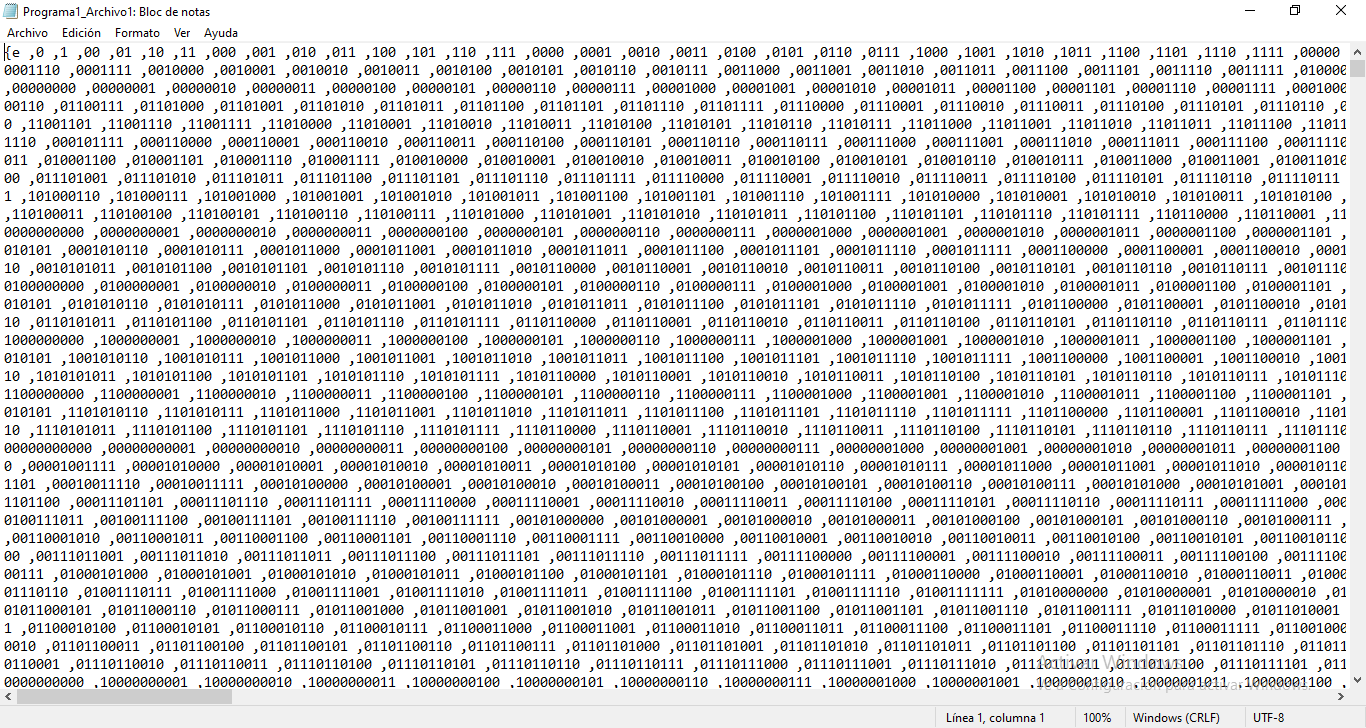
\includegraphics[width= 15cm, height= 5cm]{p1ar1.png}

Esta es la forma e la que imprime los datos separados en 32 bits
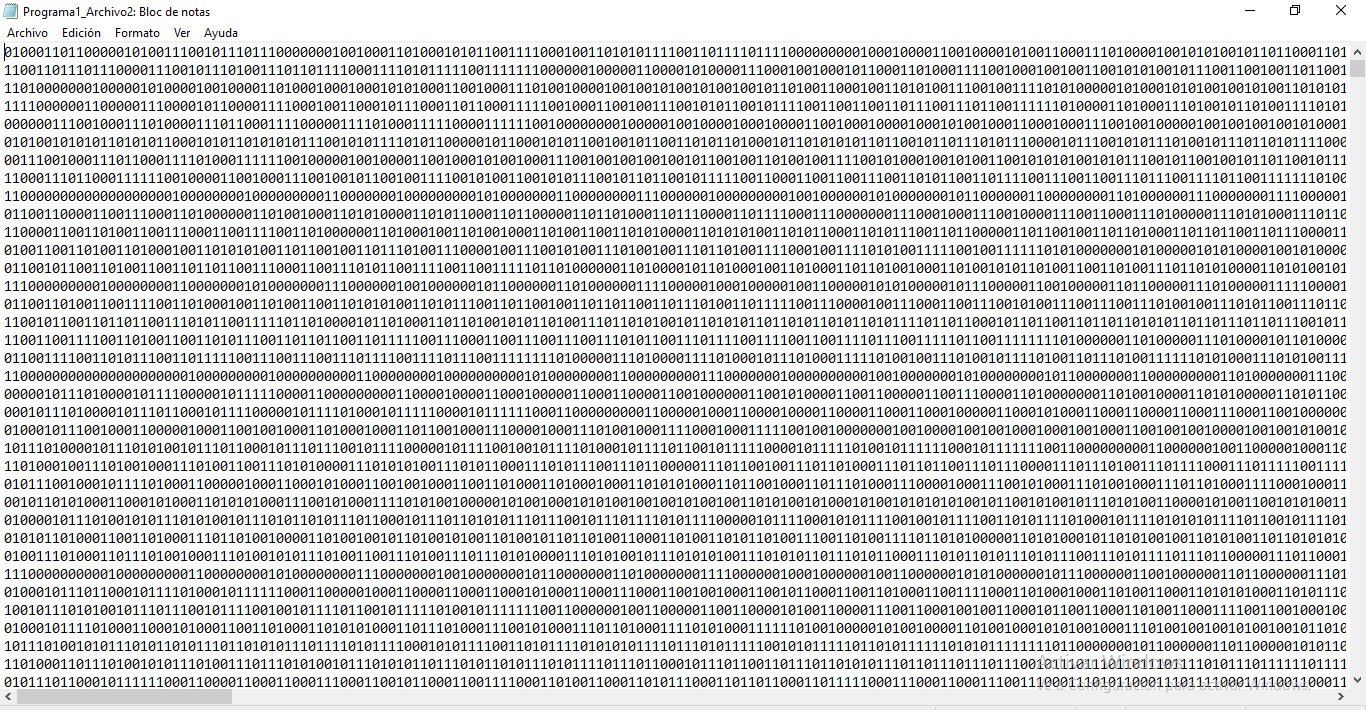
\includegraphics[width= 15cm, height= 5cm]{p1ar2.png}

Coordenadas por cantidad de 1's
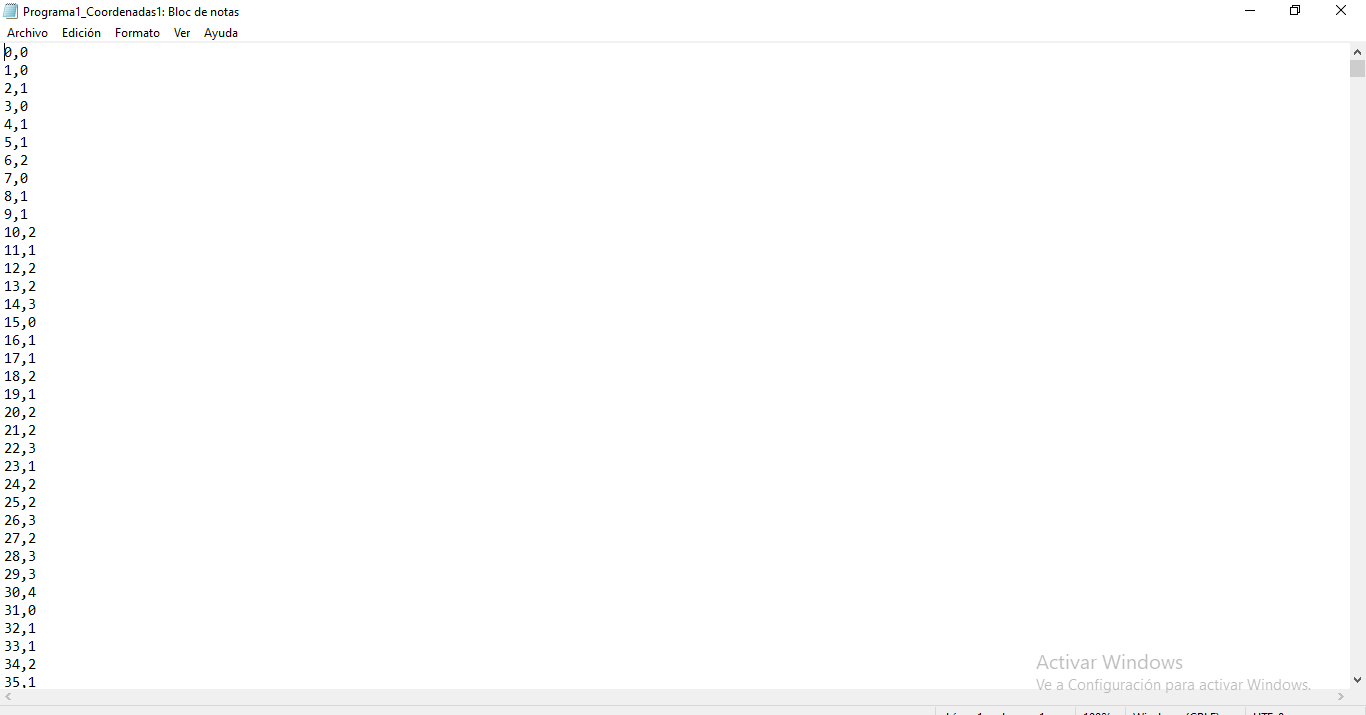
\includegraphics[width= 15cm, height= 5cm]{p1ar3.png}

Adjuntaremos imagenes de cuando n=10 (incluyendo grafica), ya que con el valor solicitado, no puede graficarse al ser muchas coordenadas

Cuando n = 10

Menu del programa
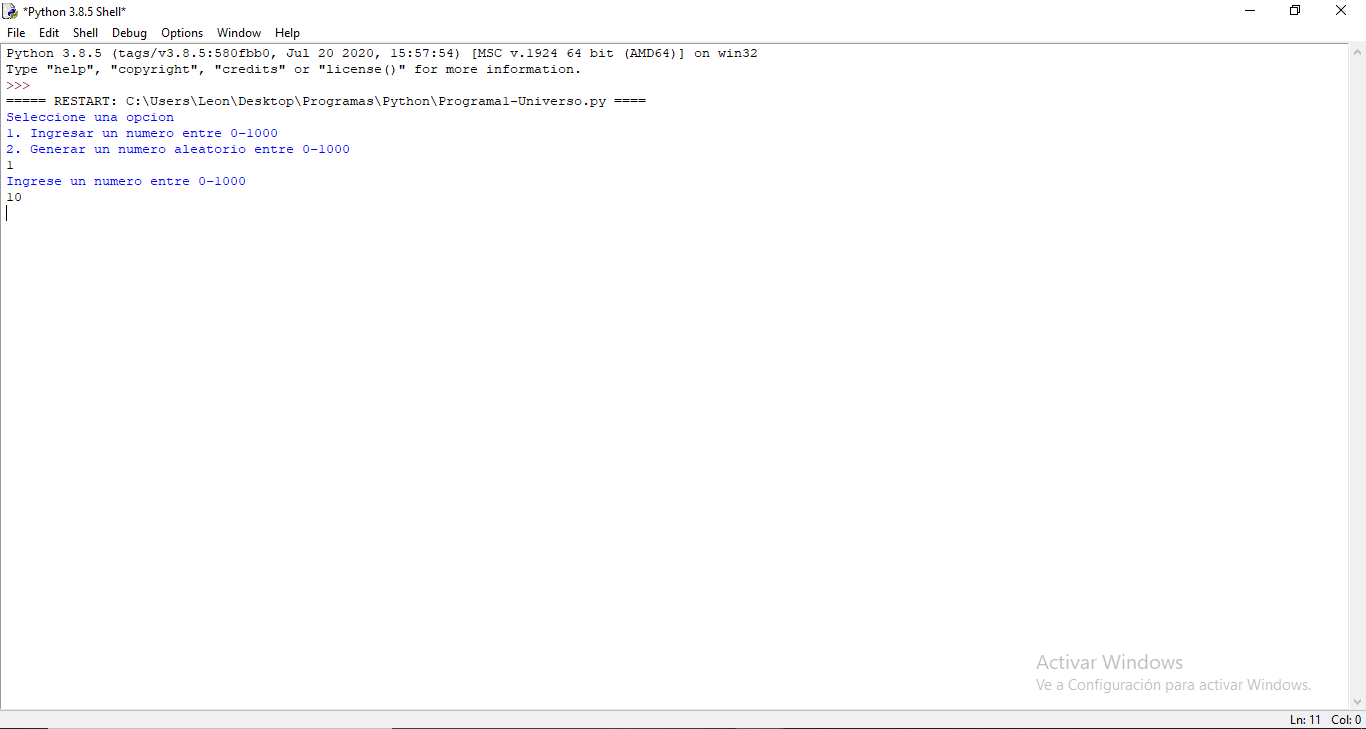
\includegraphics[width= 15cm, height= 5cm]{p1ar01.png}

Esta es la forma en la que imprime los datos en forma de conjuto
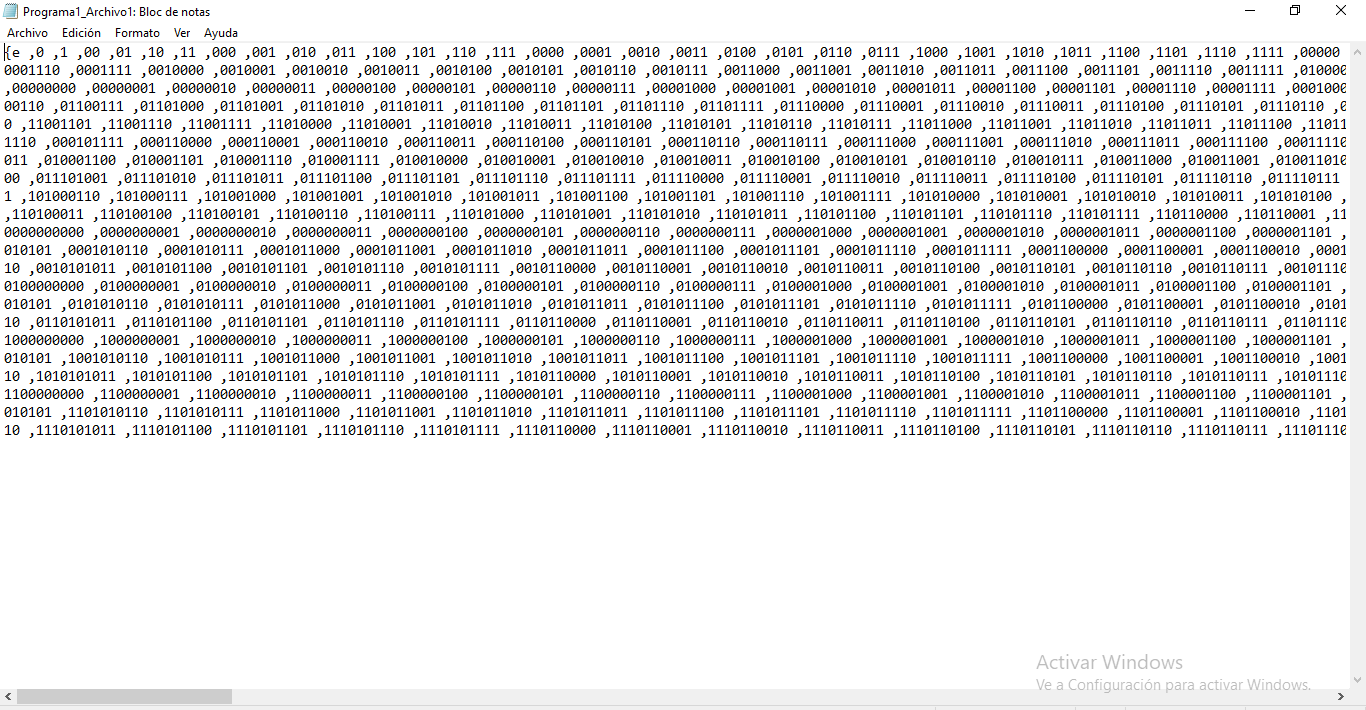
\includegraphics[width= 15cm, height= 5cm]{p1ar02.png}

Esta es la forma en la que imprime los datos separados en 32 bits
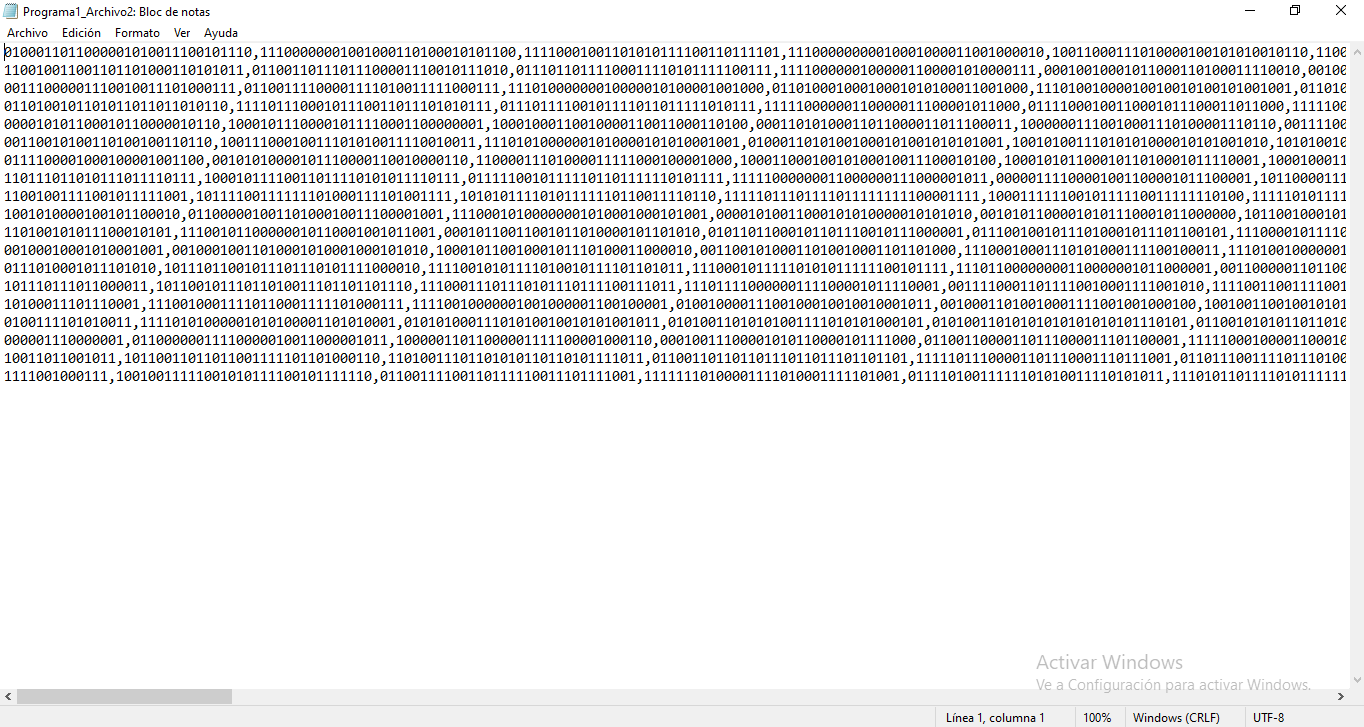
\includegraphics[width= 15cm, height= 5cm]{p1ar03.png}

Coordenadas por cantidad de 1's
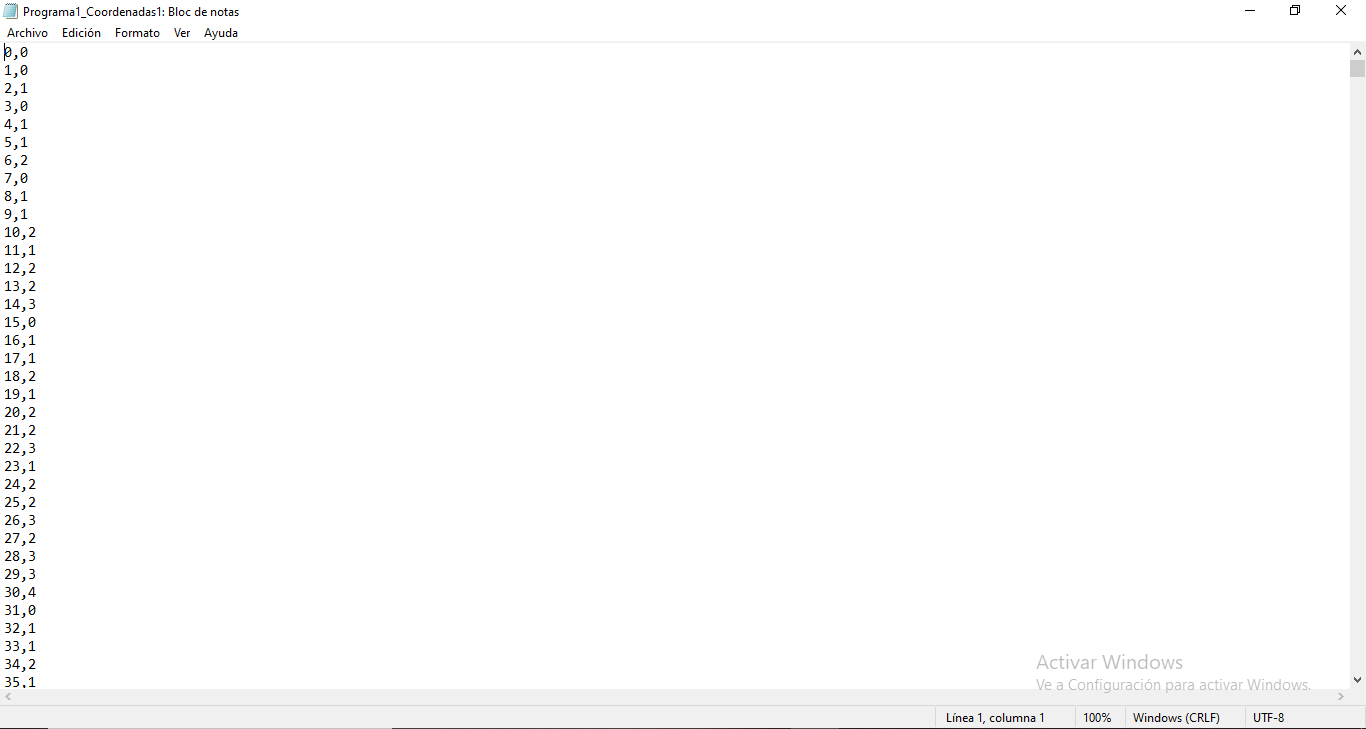
\includegraphics[width= 15cm, height= 5cm]{p1ar04.png}

Coordenadas por cantidad de 1's (32 bits)
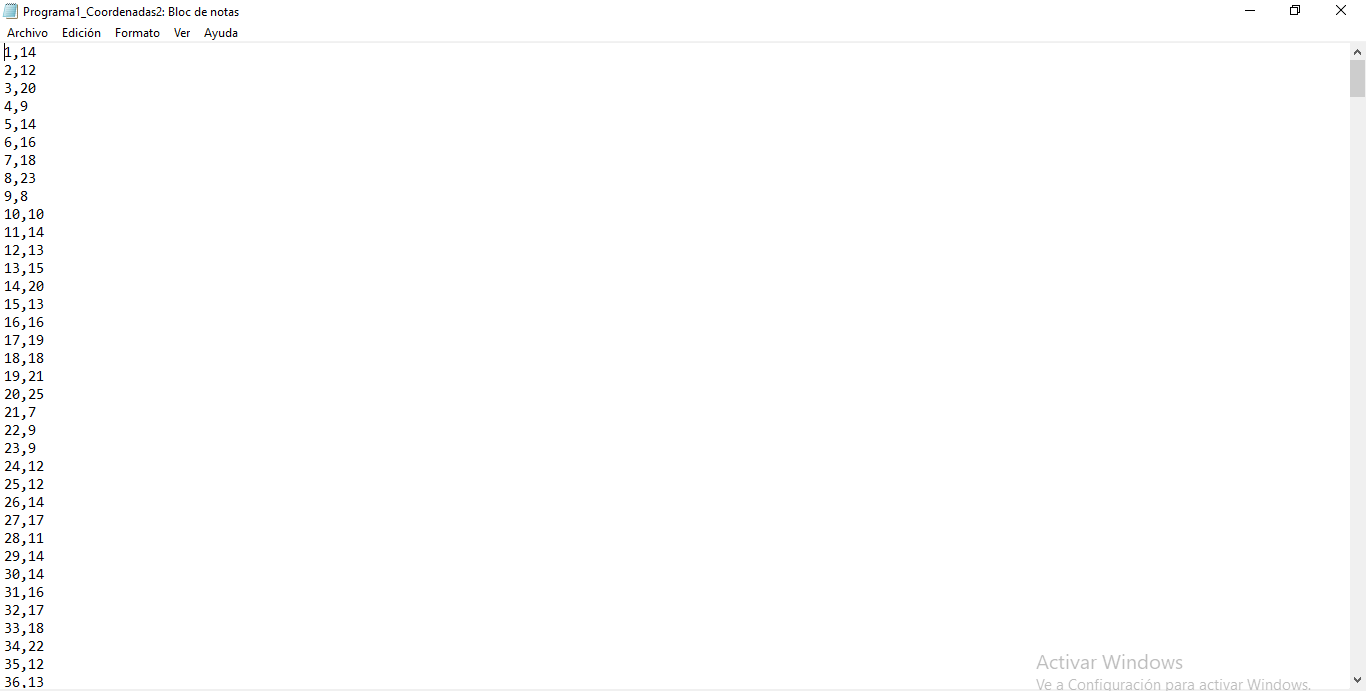
\includegraphics[width= 15cm, height= 5cm]{p1ar05.png}

Grafica por cantidad de 1's

azul = cantodad de 1's
rojo = log2
verde log10
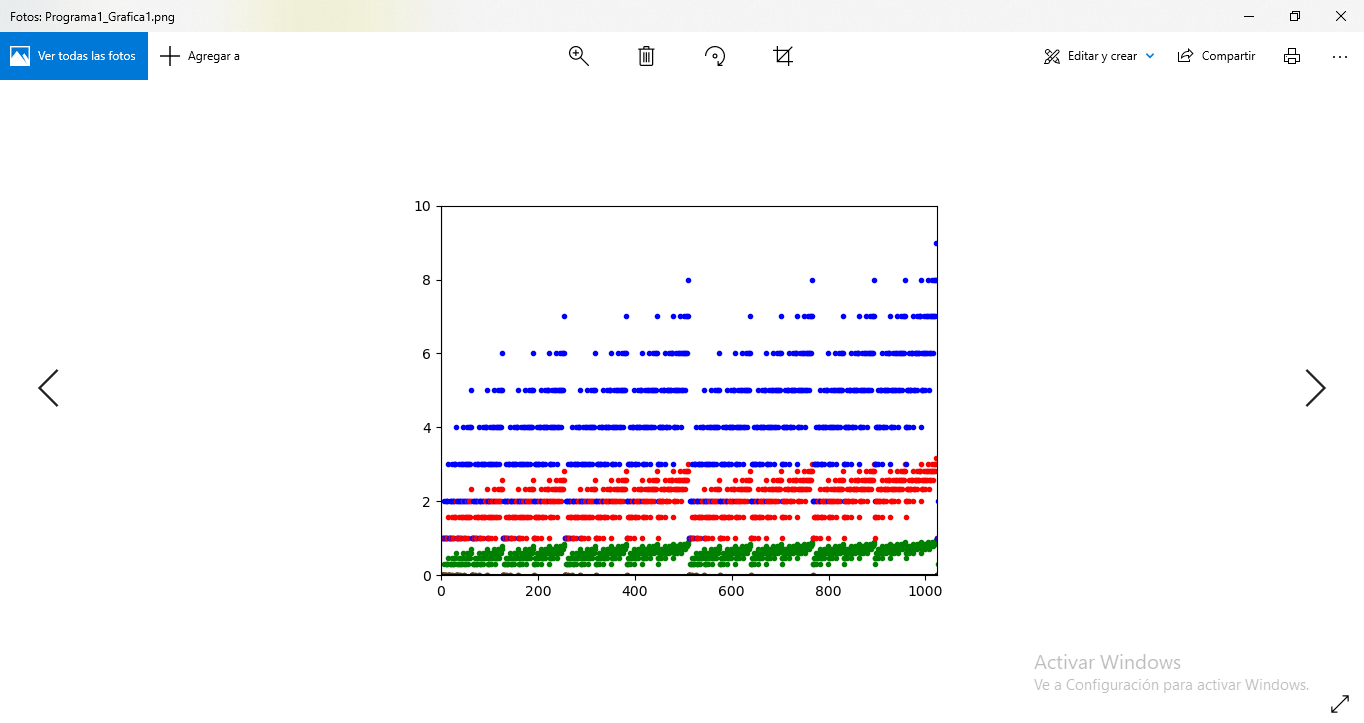
\includegraphics[width= 15cm, height= 5cm]{p1ar06.png}

azul = cantodad de 1's
rojo = log2
verde log10
Grafica por cantidad de 1's (32 bits)
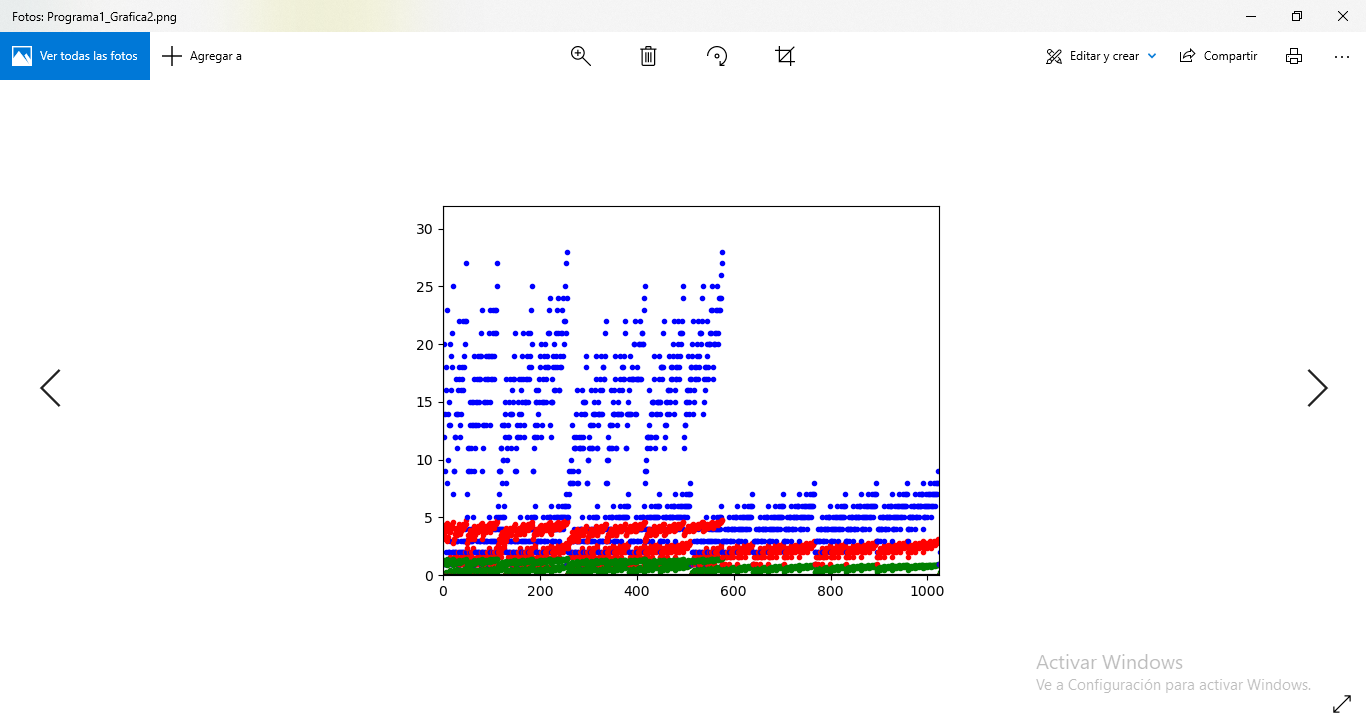
\includegraphics[width= 15cm, height= 5cm]{p1ar07.png}

\end{flushleft}
\end{document}